%&latex












\section{Introduction}



This chapter examines an instance of a PDMP, called the \textbf{$N$ particle dynamic shuffler,}  which tracks $N$ particles on the positive real line moving with velocity -1 until reaching the origin.  Upon hitting the origin, a particle is randomly redistributed back to $\mathbb{R}^+$, with respect to a probability density $p(x)$ in $\mathbb R^+$. If initial empirical densities of $N$ particles approach a limiting density $u_0(x)$, we will show that the random densities of the $N$ particle dynamic shuffler at time $\tau>0$ approach a deterministic density $u(x,\tau)$, which satisfies a weak form of a one-dimensional transport equation with source term, 
\begin{alignat}{2}  \label{pde}
\partial_\tau u(x,\tau) - \partial_x u(x,\tau) = p(x)u(0,\tau) \quad \tau, x \in \mathbb{R}^+, \\
u(x,0) = u_0(x) . \nonumber
\end{alignat}
 In this chapter, we will refer to (\ref{pde}) as the \textbf{redistribution equation}.  Regularity conditions on $u_0(x)$ and $p(x)$ largely depend on the types of solutions we seek, and will be considered throughout this chapter.

  
  


We will borrow methods from coagulation theory. For instance, consider the one-dimensional Allen-Cahn equation $\partial_t u = \partial_{xx} u+u-u^3$, which describes a coagulation process on the real line. Specifically, given an interval partition of $\mathbb R$, the smallest interval merges with its two neighbors to form a single interval, and the process continues. Menon, Niethammer, and Pego used the Allen-Cahn equation as a source of motivation in \cite{menon2010dynamics},  investigating a wide range of clustering events.  The discrete nature of these clustering phenomena  suggested that it was reasonable to seek measure-valued solutions.  Such solutions, continuous in time in the space of probability measures, were found using an intrinsic time scale based on the number of clusters in the system.  The same philosophy will be applied to (1), which will use the time scale
of the total number of visits to the origin by particles,
\begin{equation}\label{cov}
t = \int_0^{\tau} u(0,s)ds.
\end{equation}
   We should note that while the tools used in coagulation theory prove useful to this chapter, in general there is no coagulation occurring in the redistribution equation!  The total number of particles $N(\tau)= \int_{\mathbb{R}^+}u(x,\tau)dx$ is preserved, while the total mass, or first moment, $M(\tau) = \int_{\mathbb{R}^+} xu(x,\tau)dx$ can potentially change in time.

The sections of this chapter are arranged as follows.  In Section \ref{stochlimit}, we derive (\ref{pde}) as a limit of densities of the $N$ particle dynamic shuffler. This is done by exploiting the infinitesimal generator, and building a martingale approximation to (\ref{pde}). Section \ref{lapsection} derives a solution formula for (\ref{pde}) for smooth initial conditions through the Laplace transform.
We then use the change of variables (\ref{cov}) in Section \ref{meassect} to derive a measure-valued solution formula for (\ref{pde}).  A specific example is presented in  Section \ref{ptmass}, with initial data a point mass. Sections \ref{strongsection} and \ref{weaksection} prove well-posedness of weak and strong solutions for (1), meaning that the solution formulas of Sections \ref{lapsection} and \ref{meassect} are well-defined. In  Section \ref{statio}, we conclude the chapter by   providing asymptotics for $u(x,\tau)$ via the key renewal theorem from renewal theory. 


  
    
\begin{figure}
\begin{centering}
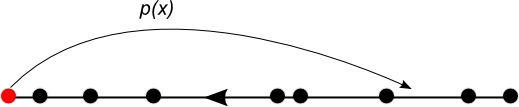
\includegraphics[width=.5\textwidth]{1dredistribution.png}
\caption{\textbf{A dynamic shuffler.} Particles (black dots) drift left with unit speed until hitting the origin, where a particle (red dot) is redistributed according to a density $p(x)$.}
\end{centering}
\end{figure}


    

 
\section{A solution via a stochastic limit}\label{stochlimit}
A discrete approximation of the behavior underlying  (\ref{pde}) can be obtained through PDMPs.  In the following section, we show the dynamic shuffler of $N$ particles is a PDMP, and then take a fluid limit as $N \rightarrow \infty$. In this limit, particle densities will converge to a weak version of (\ref{pde}).    

 

Our process is as follows.  Let particles $x_1, \dots, x_N \in \mathbb{R}^+$ be given. Each particle moves left with unit speed until a particle hits the origin.  This particle is randomly assigned a new location according to a probability distribution function $p(x) \in C^1(\mathbb{R}^+)$. The shuffler continues as before, with particles drifting until a new particle hits the origin. 

We will now show that this process can be interpreted as a PDMP.  The general theory and notation of a PDMP is discussed in  Section \ref{pdmpgenerator}.  From the viewpoint of a dynamic shuffler with $N$ particles, our state space is $E^N = \mathbb{(R^+)}^N$, with a state written as
\begin{equation}
\mathbf x = (x_1, \dots, x_N) \in E^N.
\end{equation}
 There is no need to consider disjoint copies of $E^N$. This is because particles are neither created nor destroyed, and there is only one vector field, corresponding to each particle having velocity of $-1$, namely $\mathcal X= -\sum_{i = 1}^N\frac{\partial}{\partial x_i}$.  Since all jumps  occur on the boundary of $E$, where there is a particle at the origin, we have zero jump frequency: $\lambda \equiv 0$. For an element $y \in \partial \Gamma^*$ of the form
\begin{equation}
y= \{y_1, \dots, y_{i-1},0, y_{i+1} \dots, y_N\},
\end{equation} 
the transition kernels satisfy
\begin{equation}
Q(\mathbf x,y) = \begin{cases}p(z), & \mathbf x= (y_1,\dots, y_{i-1},z,y_i,\dots, y_N), \\
0, & \hbox{otherwise.} \\
\end{cases}
\end{equation}
 We thus have a well defined PMDP  $x(t) = (x_1(t), \dots, x_N(t))$ on $E^N$. 
At each time $t >0$, we define the random empirical measure process of particle locations: 
\begin{equation}
\nu^N_t (dx) = \sum_{i = 1}^N \frac{\delta_{x_i(t)}}{N}(dx).  \nonumber
\end{equation}
Let $\phi \in C^1(\mathbb{R}^+)$, we can pair an arbitrary finite measure $\mu \in \mathcal P(\mathbb R^+) $ through integration:  
\begin{equation}
\langle \mu, \phi \rangle = \int_{\mathbb{R}^+}\phi(x) \mu(dx). \nonumber
\end{equation} A natural choice for  a functional of our PDMP is the empirical pairing $F^N(\phi):E \rightarrow \mathbb{R}^+$, defined by 
\begin{equation}
F^N(\phi)(\mathbf x) = \sum_{i = 1}^N \frac{\phi(x_i)}{N} .  \end{equation}

As a Markov process, the PDMP has an associated generator and martingale determined from Dynkin's formula. Our aim is to define a non-trivial set of test functions such that $F^N(\phi)(\mathbf x)\in \mathcal D(\mathcal A)$,    the domain of valid functionals for the infinitesimal generator $\mathcal A$.  We will use the sufficient conditions given in Theorem \ref{fourcond}.  

 
The major hurdle to show $F^N(\phi) \in \mathcal D(\mathcal A)$ is in  boundary condition (3) of Theorem 2, which is equivalent to proving 
\begin{equation}
\mathbb{E}\left[\Delta F^N(\phi)(y)\right] = 0, \quad y \in \Gamma^*,
\end{equation}
where, if a random variable $Z(y)$ is distributed in $E$ with respect to $Q(\cdot,y)$, then  
\begin{equation}
\Delta F(y) = F(Z(y))-F(y).
\end{equation}
In order for  condition (3) to hold, we must equate the value of a particle at the origin,  $\phi(0),$ with its expected value when it is redistributed back to $\mathbb R^+$. We thus use the space of test functions  
\begin{equation}
\mathcal  C  \ = \left\{\phi \in C^1(\mathbb{R}^+) \mid \phi(0) = \int_0^\infty \phi(x)p(x)dx, \quad \|\phi'\|_\infty<\infty \right\} . \end{equation}
It's straightforward to show, using the regularity of $\phi \in \mathcal C$, that our empirical functional $F^N(\phi)$,  is  in the domain $\mathcal D(\mathcal A)$. Vector fields satisfy, by the chain rule,
\begin{equation}
\mathcal X(F^{N}(\phi)(\mathbf x)) = \sum_{i = 1}^{N}-\frac{\partial}{\partial x_i}\frac{\phi(x_i)}{N} = -\sum_{p_i \in T_k} \frac{\phi'(x_i)}{N} 
 = -\langle \nu_s^N, \phi'  \rangle. 
\end{equation}
   The martingale $M_\phi^N(t)$ associated with $F^N(\phi)$ given in (\ref{generator}) and (\ref{martingale}),   then satisfies 
\begin{equation}\label{marty}
M^N_\phi(t) = \langle \nu_t^N,\phi \rangle- \langle \nu_0^N,\phi \rangle- \int_0^t \langle \nu_s^N,\phi' \rangle ds . 
\end{equation}



   


It is of note that if we allow for initial empirical data to converge to measures with jumps in its cumulative distribution function, then we should not expect convergence in the $J1$ topology. Indeed, if we initial empirical densities densities that approach a point mass,  redistribution of particles concentrate during increasingly small time intervals. During this interval, the value $F^{N}(\phi)(X(t))$ forms an approximately continuous ``monotone staircase" between $\phi(0)$ and $\mathbb{E}[\phi(X)]$ whose jumps do not approach that of the limiting function (see Fig. \ref{topcounter})

The right topology to invoke in this case is the Skorokhod M1 topology, a weaker version of the J1 topology. Convergence of functions in this case is characterized by measuring the distance between the completed graphs of cadlag functions.  In particular, continuous functions can approximate a function with jumps.  We refer the reader to \cite{whitt2002stochastic} for a rigorous explanation of the $M1$ topology, as well as its relation to the $J1$ topology.   We withhold a discussion of $M1$ convergence of the redistribution equation for now, and hope to address the issue in future work.  Thus, in this exposition, our initial empirical measures will approach nonatomic measures.  
\begin{figure}
\begin{centering}
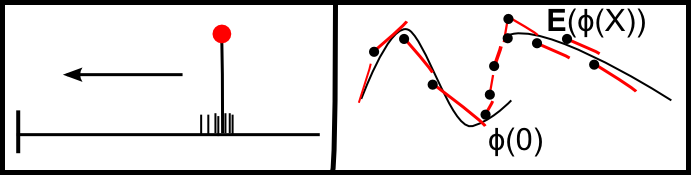
\includegraphics[width=.5\textwidth]{topcounter.png} 
\caption{\textbf{M1 convergence of measure valued initial data.}  \textbf{Left: }Particles (small vertical segments) approximating a point mass (segment with red dot) drift toward the origin. \textbf{Right:} The value of $F(\phi)(x)$ before and after particles hit the origin. As the number of particles grows, their jumps form a ``monotone staircase" connecting the jump of the limiting functional.}\label{topcounter}
\end{centering}
\end{figure}





\subsection{Convergence of empirical processes}

 We are now ready to state our main theorem.  It may be seen as a  law of large numbers limit for random empirical densities. 

\begin{theorem}\label{pdmpproof}
Suppose we have weak convergence of initial empirical measures $\nu_0^n \rightarrow \nu_0 $, where $\nu_0 $ is nonatomic.  Then the random measure process $\nu_t^N$ converges to a deterministic limit $\nu_t$ under the Skorokhod topology $\mathbb D([0,t], \mathcal P(\mathbb{R}^+))$. The limiting measure satisfies the kinetic equation
\begin{equation}\label{limeq1}
0= \langle \nu_t,\phi \rangle- \langle \nu_0,\phi \rangle- \int_0^t \langle \nu_s,\phi' \rangle ds \quad 
\end{equation}
for every $\phi \in \mathcal C$.

\end{theorem}
The following two lemmas will help in establishing tightness \cite{roelly1986criterion,joffe1986weak}.


\begin{lem}\label{Cap}
Let $T>0$. A sequence $\nu_k(t)$ in $\mathbb D([0,T], \mathcal M(\mathbb{R}^+))$ is tight if and only if the sequence of functions $\langle \phi, \nu_k(t) \rangle$ is tight in $\mathbb D([0,T],\mathbb{R}^+)$ for all $\phi \in C_b(\mathbb R^+)$.
\end{lem}



\begin{theorem}\label{Ald}
 (\textbf{Aldous' conditions}) Let $T>0$. A sequence of stochastic processes $X_n(t)$ is tight in  $\mathbb D([0,T],\mathbb{R}^+)$ if the following two conditions hold:
\begin{enumerate}
\item For all rational $t \in [0,T)$ and for all $\varepsilon > 0$, there exists an $L>0$ such that
\begin{equation}
\sup_{n>0} \mathbb{P}(|X_n(t)|>L) \le \varepsilon.
\end{equation}
\item For jump times $\tau_1, \dots, \tau_{m(t)}$, then for all $\varepsilon >0$,
\begin{equation}
\lim_{r \rightarrow 0} \limsup_{n \rightarrow \infty} \sup_{s<r,\tau_{i}}  \mathbb P(|X_n((\tau_i+s) \wedge T) - X_n(\tau_i)| > \varepsilon) = 0.
\end{equation}
\end{enumerate}
\end{theorem} 

Combining the two statements, we need to show that, for a fixed $\phi \in C_b(\mathbb R^+),$ the sequence of random variables $X_n(t) = \langle \phi, \nu_t^N \rangle $ satisfies Aldous' conditions. 



Before showing the next lemma, we define the set of intervals of width less than $\delta>0$:
\begin{equation}
I_\delta = \{(a,b)\subset \mathbb{R}^+, b-a<\delta\}.
\end{equation}
\begin{lem}\label{tech} Let $T>0$.  Suppose $\nu_0^N \rightarrow \nu_0$ weakly, and $\nu_0$ is nonatomic. Then for all $\eta > 0$, 
\begin{equation}\label{paccon}
 \lim_{\delta \rightarrow 0} \sup_{I \in I_\delta}\limsup_n \sup_{t \in [0,T]}\mathbb P(\nu_t^N(I) >\eta)) = 0 .
\end{equation}
\end{lem}

\begin{proof}
Let $\eta > 0$. For $T = 0$, we have that (\ref{paccon}) follows from the fact that $\nu_0$ is nonatomic.
% \begin{equation}\label{zerocase}
% \lim_{\delta \rightarrow 0}\limsup_n\nu_0^n(I_\delta) = 0
% \end{equation}
% 
% for all $\delta$ intervals $I_\delta$.
% 
% Suppose, for contradiction, that this were not the case.  This means for each $M \in \mathbb{N}$, there is a subsequence $\nu_0^{n_k^M}$ and intervals $I_{1/M}$ that satisfy $\limsup_{n_k^M}\nu_0^{n_k^M}(I_{1/M}) \ge \eta$, which implies $\lim_{n\rightarrow \infty} \nu_0^n(I_{1/M}) \ge \eta$.  Let $L>0$ so that $\nu_0([L,\infty))= \eta/2.$  Note that only finitely many sets $I_{1/M}$ lie in $[L,\infty)$.  Otherwise, 
%  
%  $$1-\eta/2 = \nu_0([0,L)) = \lim_{n\rightarrow \infty} \nu_0^n([0,L))\le1-\eta,$$
%  a contradiction.  Now let $p_M$ denote the centers of the intervals $I_{1/M}$.  Since $[0,L]$ is compact, we have a cluster point $p$ of the sequence $p_k$ . Therefore, any interval containing $p$ contains infinitely many intervals $I_{1/M}$. We then have
%  
%  $$0 = \nu_0(p) = \lim_{n \rightarrow \infty} \nu_0([p-1/n,p+1/n]) = \lim_{n \rightarrow \infty} \lim_{k \rightarrow \infty} C^k_0([p-1/n,p+1/n])>\eta,$$
% which is our desired contradiction.  Thus (\ref{zerocase}) holds.

We now show (\ref{paccon}) for $s \in \mathbb{R}^+$. For $S\subset \mathbb{R}$  , we denote $S+s = \{x \in \mathbb{R}|x-s \in S\}$. Now let $T>0$.  For $t\in [0,T]$, $\nu_t^N(I)$ is equal to the sum of $\nu_0^n(I+t)$ and the sum of masses that are redistributed to $I+t-s$ at time $s$.

To estimate redistribution probabilities, we focus on the location of a single particle $x(t)$ for $t \in [0,T].$ Let 
\begin{equation}
M_\delta = \sup_{x \in \mathbb R^+} \int_x^{x+\delta}p(s)ds.
\end{equation}
Note that because $p \in L^1(\mathbb{R}^+)$, $M_\delta \rightarrow 0$ as $\delta \rightarrow 0$. Now,  the probability of $x(t) \in I$ is bounded by the number of jumps that $x(t)$ undergoes, multiplied by the probability that the next jump lands in the correct $\delta$ interval, or
\begin{eqnarray}
\mathbb{P}(x(t) \in I) \le \sum_{k = 0}^\infty\mathbb{P}(x(t) \hbox{ has $k$ jumps})M_\delta\\
\le M_\delta\sum_{k = 0}^\infty \mathbb{P} \left(\sum_{i = 1}^k X_i <t)\right),\nonumber
\end{eqnarray}
where $X_i, i \in \mathbb N$ is a sequence of i.i.d random variables distributed with respect to $p(x)$.
A Chernoff-type bound shows that the sum over $k$ converges.  Indeed, we have
\begin{eqnarray}\label{chernoff}\mathbb{P} \left(\sum_{i = 1}^k X_i <t\right) =\mathbb{P} \left(\exp\left(-\sum_{i = 1}^k X_i) \right)>\exp(-t)\right)\\
\le e^{t}\mathbb{E}[e^{-X_1}]^k, \quad k \in \mathbb N,\label{expseries} \nonumber
\end{eqnarray}
by Markov's inequality. The series of  terms (\ref{expseries})  is then  summable over $k$ to a finite constant, denoted $K$.
As particles $x_1(t), \dots,x_n(t)$ behave independently, we now have an estimate for  $\nu_t^N(I)$, given by 
\begin{equation}
 \mathbb{E}[\nu_t^N(I)] \le Ke^tM_\delta. \nonumber
\end{equation}
But then we have, from Markov's inequality,
\begin{eqnarray}
\lefteqn{\sup_{t \in [0,T]}\mathbb{P}( \nu_t^N(I)>\eta)}\\ &&\le  \sup_{t \in [0,T]}\mathbb{P}( \nu_t^N(I)>\eta)  
 \le\sup_{t \in [0,T]}\frac{\mathbb{E}[ \nu_t^N(I)]}{\eta}\nonumber\\&&\le \frac{Ke^TM_\delta}{\eta}  \ \rightarrow 0\quad  \hbox{ as  } \delta \rightarrow 0 \nonumber
\end{eqnarray}
\end{proof}

From here the proof for Aldous' conditions is straightforward.
\begin{theorem} For $\phi \in \mathcal C$, the Aldous conditions in  Theorem \ref{Ald} hold for $\langle\nu, \phi\rangle$
\end{theorem}
\begin{proof}

Condition 1: This follows trivially since $\langle\phi, \nu_t^N\rangle \le \|\phi \|_\infty$, meaning that $L = \|\phi\|_\infty$ satisfies Condition 1.

Condition 2:   We have
\begin{eqnarray}
|\langle\phi,\nu_{\tau+s \wedge T}^N\rangle \  - \langle\phi,\nu_{\tau}^N\rangle| = \left| \int_{\mathbb{R}^+}\phi(x) (\nu_{\tau+s\wedge T}^N - \nu_\tau^N)(dx)\right | \\
\le \left | \int_s^\infty (\phi(x-s)-\phi(x))\nu_\tau^N(dx)  \right|+\|\phi\|_\infty \nu_{\tau}^N([0,s]). \nonumber
\end{eqnarray}
Since $\phi$ is continuous, the first term approaches 0 as $s \rightarrow 0$, and by Lemma \ref{tech}, we have that for any $\varepsilon >0$, 
  \begin{equation}
 \lim_{s \rightarrow 0}\limsup_N\sup_{\tau \in [0,T]}\mathbb P( \nu _{\tau}^N([0,s])>\varepsilon/\|\phi\|_\infty) = 0,     
\end{equation} 

which verifies Condition (2), and completes our proof.
\end{proof}

We will now take care of the martingale term, which we can show is bounded in the local uniform metric:


\begin{theorem}\label{martyproof}
The martingale term $M^\phi_N $ in (\ref{marty}) is bounded by 
\begin{equation}
\mathbb{E}\left[\sup_{s \in [0,t]}(M_N^\phi(s))\right] \le \frac{Be^{t/2}\|\phi\|_\infty}{\sqrt N},
\end{equation}
where $B$ is a constant determined by a summable series.
\end{theorem}

\begin{proof} 
We first note that
\begin{equation}
|\Delta M_N^\phi(t) |= |M_N^\phi(t)-M_N^\phi(t^-)| = |\Delta\langle \nu_t^N,\phi\rangle| \le \frac{2\|\phi\|_\infty}N 
\end{equation}
It then follows, for $d_N(t)$ denoting jump times $\tau_1, \dots, \tau_{d_N(t)}$, that
\begin{eqnarray}
\mathbb E\left[M_N^\phi(t)^2\right] = \mathbb{E}\left[\sum_{i = 1}^{d_N(t)}\Delta M_N^\phi(\tau_i)^2\right]\\
\le\frac{4\|\phi\|_\infty^2}{N^2} \mathbb{E}[d_N(t)]\nonumber
\end{eqnarray}
Here we again appeal to Chernoff bounds in (\ref{chernoff}) to help estimate the total number of jumps that occur. Let $x(t)$ denote the stochastic process tracking a tagged  particle.  This gives us 
 \begin{eqnarray}
 \mathbb{E}[\#\{\hbox{jumps for } p(t)\}] = \sum_{k = 0}^\infty k \mathbb{P}(p(t) \hbox{ jumps $k$ times})\\
\le k\mathbb{P}\left(\sum_{i = 0}^k X_i \le t\right)\le e^t \sum_{k = 0}^\infty k\mathbb{E}[e^{-X_1}]^k\le Ce^t \nonumber 
\end{eqnarray} 
for some constant $C$.  This gives us $\mathbb E[d_N(t)] \le CNe^t$, meaning
\begin{equation}
\mathbb{E}[M_N^\phi(t)^2] \le  \frac{4Ce^t\|\phi\|_\infty^2}{N}.
\end{equation}

Now, using Doob's inequality, we obtain
\begin{equation}
\mathbb{E}\left[\sup_{s \le t}|M_N^\phi(s)|\right]^2 \le \mathbb E\left[\sup_{s \le t} M_N^\phi(s)^2\right] \le 4\mathbb E[M_N^\phi(t)^2]
\end{equation}
Setting $B =4 \sqrt C$ then gives our desired result.
\end{proof}

Since we have shown tightness, we can extract a subsequence $\nu_t^{N_k} \rightarrow \nu_t$ in the Skorokhod J1 topology.  Furthermore, since local uniform  convergence is stronger than convergence under the Skorokhod topology, we also have $M_{N_k}^\phi(t) \rightarrow 0$ in $\mathbb D([0,T], \mathbb{R})$.  Thus our limiting measure $\nu_t$ satisfies equation (\ref{limeq1}).

We now finish the proof of Theorem \ref{pdmpproof} by showing uniqueness of limits.  This will be done by approximating the measure processes PDMP $X^N(t)$ by processes $X^{N,\varepsilon}(t) = (x_1^{N,\varepsilon}(t), \dots, x_N^{N,\varepsilon}(t))$ with perturbed redistribution probabilities $p_\varepsilon(t)$, given by
\begin{equation}
p_\varepsilon(x) = \begin{cases}0 & x \in [0,\varepsilon]  \\
\frac{p(x)}{\int_\varepsilon^\infty p(y)dy} & x >\varepsilon.\\
\end{cases}
\end{equation}
These redistributions are probabilities of a particle redistributed with respect to $p$, conditioned on being redistributed in $[\varepsilon, \infty)$.  Suppose now that for time $t \in [0,\varepsilon]$, we have random processes $\nu_t^{N,\varepsilon}$ given by  
\begin{equation}
\nu_t^{N,\varepsilon} = \sum_{i = 1}^N \frac{\delta_{x_i^{N,\varepsilon}(t)}}{N}. \end{equation}
If for some nonatomic $\nu^{\varepsilon}$ we have convergence of initial measures $\nu^{N,\varepsilon} \rightarrow \nu^\varepsilon$ in the $J1$ topology, then there is a unique deterministic measure valued limit $\nu_t^\varepsilon$ of $\nu_t^{N, \varepsilon}$.  For any open interval $A$, 
\begin{equation}
\nu_t^\varepsilon(A) = \nu_0^\varepsilon(A+t) +\int_0^t\int_Ap_\varepsilon(x+t-s)dxdF_{\nu_0^\varepsilon}(s),
\end{equation}
where $F_{\nu_0^\varepsilon}(s)$ is the cumulative distribution function of $\nu_0^\varepsilon$ for time $s \in [0,\varepsilon)$.  That we have such a deterministic formula comes from the fact that when $t \in [0,\varepsilon]$, particles only redistribute once. Thus, the total amount of  redistributed mass at time $t$ is exactly equal to $F_{\nu^\varepsilon(t)}$. The uniqueness actually extends for all time $t \in [0,\infty)$, since we can extend our unique solution to time $2\varepsilon$ by setting initial conditions equal to $\nu^\varepsilon_\varepsilon$, and so forth. 

Let $L^N_\varepsilon(t)$ and $|L^N_\varepsilon(t)|$ denote the support and number, respectively,  of particles which at some time hit the origin and are redistributed to $[0,\varepsilon]$ in time $[0,t]$. We now split the process $\nu^N_t$ by which   particles are in $L^N_\varepsilon(t):$
   \begin{equation}\label{meassplit}
  \nu_t^N =\frac{N-|L_\varepsilon^N(t)|}{N} \sum_{a_i^{N}(t) \notin L_\varepsilon^N(t)}\frac{\delta_{a_i^N(t)}}{N-|L_\varepsilon^N(t)|}+ \sum_{a_i^{N}(t) \in L_\varepsilon^N(t)}\frac{\delta_{a_i(t)}}{N}.\\ \end{equation}
Now we use the martingale bounds from Theorem \ref{martyproof} to see that
\begin{eqnarray}
  \mathbb{E}[\frac{|L_\varepsilon^N(t)|}{N}]\le \frac{\mathbb{E}[d_N(t)]}{N}
\int_0^\varepsilon p(x)\\\le  Be^t \int_0^\varepsilon p(x) \rightarrow 0 \quad   \quad \hbox{ as }\varepsilon\rightarrow 0\nonumber
\end{eqnarray}
 Therefore, the second term in (\ref{meassplit}) approaches 0 in $L^1$. Notice, however, that particles not in $L_\varepsilon^N(t)$ are distributed with respect to  $p_\varepsilon$. Thus, we have , for identical initial empirical measures $\nu_0^N =\nu_0^{N, \varepsilon}$, then for any open interval $A \subset \mathbb{R}^+$, we have
\begin{equation}
\mathbb{E}\left[\sup_{s \in [0,t]}| \nu^N_s(A)- \nu_s^{N,\varepsilon}(A)|\right] \rightarrow 0 \quad \hbox{ as } \varepsilon \rightarrow 0
\end{equation}

For subsequences $n_1(N)$ and $n_2(N)$ with $n_i(N)\rightarrow \infty$ as $N\rightarrow \infty$ for $i = 1,2$, suppose that we had two converging subsequences $\nu^{n_1(N)}_t\rightarrow  \nu_t$ and $\nu_t^{n_2(N)}\rightarrow \tilde \nu_t$ in $\mathcal P(\mathbb{R}^+)$. Applying the triangle inequality then yields, 
 \begin{eqnarray}
 \lefteqn{\mathbb{E}\left[\sup_{s \in [0,t]}|\nu_s(A)-\tilde \nu_s(A)|\right]}\\
 &&\le \mathbb{E}\left[\sup_{s \in [0,t]}|\nu_s(A)- \nu_s^{n_1(N)}(A)|\right]+\mathbb{E}\left[\sup_{s \in [0,t]}|\tilde \nu_s(A)- \nu_s^{n_2(N)}(A)|\right]\nonumber\\
&&+\mathbb{E}\left[\sup_{s \in [0,t]}|\nu_s^{n_1(N)}(A)-\nu_s^{n_1(N),\varepsilon}(A) |\right]+\mathbb{E}\left[\sup_{s \in [0,t]}|\nu_s^{n_2(N)}(A)-\nu_s^{n_2(N),\varepsilon}(A) |\right] \nonumber\\
&&+\mathbb{E}\left[\sup_{s \in [0,t]}| \nu_s^{n_1(N),\varepsilon}(A)-\nu_s^{n_2(N),\varepsilon}(A) |\right]. \nonumber
\end{eqnarray} 
   As $n$ and $\varepsilon$ were arbitrary, if we take limits of $N \rightarrow \infty$, and then $\varepsilon \rightarrow 0$ , we see that in fact $\nu_s = \tilde \nu_s$. 








\section{A solution via the Laplace transform}\label{lapsection}

The goal for the rest of this chapter is to generalize (\ref{pde}) for a larger class of initial conditions, and prove a basic result about a universal attractor.  Our hope is that such an analysis will highlight the use of several techniques that may be utilized for more complicated PDMPs. The existence of universal attractors is a sought after problem in coarsening systems, such as Smoluchowski's coagulation equation \cite{menon2004approach} and grain boundary coarsening \cite{her12}. 

We begin our study of (\ref{pde}) by noting that the rate of redistribution in (\ref{pde}) is given by the local quantity $u(0,\tau)$.  This, if not already evident, becomes clear when we integrate along characteristics $x(\tau) = x_0-\tau$, giving us the integral form of the redistribution equation:
\begin{equation}\label{intsol}
u(x,\tau) = u_0(x+\tau) +\int_0^\tau p(x+\tau-s)u(0,s)ds. 
\end{equation}
Thus, well-posedness of (\ref{intsol}) ultimately depends on the behavior of $u(0,s)$.
Throughout this chapter, we'll use the Laplace transform  
\begin{equation} v(q,\tau) := \int_{\mathbb{R^+}}e^{-qx}u(x,\tau)dx. 
\end{equation}
We use the identity for the Laplace transform of $u_x$,  
\begin{eqnarray}\label{lapux}
\int_{\mathbb{R^+}}e^{-qx}u_x(x,\tau)dx = \int_{\mathbb{R^+}}\partial_x(e^{-qx}u(x,\tau))-\partial_x(e^{-qx})u(x,\tau)dx\\
 = q\int_{\mathbb{R^+}}e^{-qx}u(x,\tau)dx - u(0,\tau) = qv-u(0,\tau) \nonumber 
 \end{eqnarray}
 Denoting $\mathcal L(f)$ as the Laplace transform of  $f$ ,  (\ref{lapux}) then gives us
\begin{align*}
\mathcal{L}(u_\tau-u_x) = \dot v-qv+u(0,\tau), \hbox{ and }   \\
\mathcal L(p(x)u(0,\tau)) = \bar P(q)u(0,\tau),
\end{align*}
where we define $ \bar P(q)$ to be the Laplace transform of $p(x)$.  We now have (\ref{pde}) in the Laplace variable $v$,
\begin{equation}
\dot v -qv = (\bar P(q)-1)u(0,\tau),
\end{equation}
which may be  easily solved for $v$, giving us
\begin{equation}\label{lapsol}
v(q,\tau) = e^{q\tau}v_0(q)+(\bar P(q)-1)\int_0^\tau e^{q(\tau-s)}u(0,s)ds.
\end{equation}
This solution is similar to (\ref{intsol}), but here we can use Laplace inversion to extract a formula for $u(0,s)$.  As we are taking the Laplace transform of a probability density, we have that $|v(q,\tau)|<1$ for $\tau>0, q \in \mathbb{C}_+$. Thus $v(q,\tau)e^{-q\tau} \rightarrow 0$ as $t\rightarrow \infty$.  We then can obtain, from the $\tau\rightarrow \infty$ limit of (\ref{lapsol}),
\begin{equation}\label{fpreinv}
\frac{1}{1-\bar P(q)}v_0(q) = \int_{\mathbb{R^+}}e^{-qs}u(0,s)ds. \nonumber
\end{equation}
Written this way, we now have a formula for $u(0,\tau)$ based on the initial data.
Notice that the left hand side is a Laplace transform in the spatial variable, whereas the right hand side is a Laplace transform in time of $u(0,\tau)$. 

We now define  the trace $\alpha(s) = u(0,s)$, and the measure describing the total number of redistribution
\begin{equation}
 A(ds) := \alpha(s)ds.\nonumber
\end{equation}
An application of the Fourier inversion formula now gives us 
 \begin{equation}\label{solalpha}
\alpha(\tau) = \frac 1{2\pi}\int_\mathbb{R} e^{i\xi \tau} \frac {1}{1-\bar P(i\xi)} v_0(i\xi)d\xi.
\end{equation} 
We can apply the convolution theorem for Fourier transforms to obtain
\begin{equation}\label{alphainit}
\alpha(\tau) = \int_{\mathbb{R}^+}K(\tau-x)u_0(x)dx,
\end{equation}
where 
\begin{equation}
K(x) = \mathcal F^{-1}\left(\frac{1}{1-\bar P(q)}\right)(x),\nonumber
\end{equation}and $\mathcal F^{-1}(f)$ is the Fourier inverse of a function $f$.
The main point here is that we now have a solution formula for $\alpha(\tau)$ based only on initial data, showing that well-posedness of $(\ref{pde})$ is equivalent to   (\ref{solalpha}) being well-defined. 
\section{A measure valued solution formula }\label{meassect}

We now seek measure valued solutions via a change of variables of the total amount of redistributed mass.  For $\tau$ denoting the normal time coordinates, we use $t$ to denote the change of variables given by
\begin{equation}
t = \int_0^\tau \alpha(s)ds:= A(\tau).
\end{equation}
We'll first reformulate (\ref{pde}) in terms of measures.  Let 
\begin{equation}
\bar F_\tau(q) = \int_0^\infty e^{-qx} f(x,\tau)dx = \int_0^\infty e^{-qx} F_\tau(dx).
\end{equation}
This gives us the ODE 
\begin{equation}\label{measode}
\dot{\bar F}- qF = (1-\bar P(q))\alpha(\tau),
\end{equation}
and solution formula
\begin{equation}
\bar F_\tau(q)e^{-q\tau}- \bar F_0(q) = (\bar P(q)-1)\int_0^\tau e^{-qs}\alpha(s)ds
\end{equation}
We have, a priori, that 
\begin{equation}
|\bar F_\tau(q)| \le 1 \quad q \in \mathbb C_+,
\end{equation}
thus  $\bar F_\tau(q)e^{-qz} \rightarrow 0$ as $\tau \rightarrow \infty$.  We therefore obtain
\begin{equation}\label{fundrel}
\bar \alpha (q) = \frac{1}{1-\bar P(q)}\bar F_0(q).
\end{equation}
Equation (\ref{fundrel}) is of great importance for the rest of this chapter, as it gives us a simple relation between initial data and our change of scale.  

Again, through the convolution theorem, we can write the trace as
\begin{equation}
\alpha(s) = \int_0^\infty K(s-x)F_0(dx)
\end{equation}
Assuming $\alpha >0$ (we'll give conditions for this in Corollary \ref{cor1}), we have that $A(\tau)$ is strictly increasing, and that 
\begin{equation}
\frac{dt}{d\tau} = \alpha(\tau).
\end{equation}
  
Our ODE (\ref{measode}) is transformed as 
\begin{eqnarray}
\frac d{d\tau}(e^{-q\tau}\bar F(q)) = (1-\bar P(q))(e^{-q\tau}\alpha(\tau)) \\  \Rightarrow \frac 1{\alpha(z)}\frac d{d\tau}(e^{-q \tau}\bar F) =(1-\bar P(q))e^{-q\tau}\nonumber.
\end{eqnarray}
From the chain rule, this is equivalent to
\begin{equation}
\frac d{dt}(e^{-q \tau(t)}\bar F) =(1-\bar P(q))e^{-q\tau(t)}.
\end{equation}
This in turn gives us the solution formula
\begin{equation}\label{solutionform}
\bar F_t(q)e^{-q\tau(t)} - \bar F_0(q) = (1-\bar P(q))\int_0^t e^{-q\tau(s)}ds.
\end{equation}
Since $\tau(t) \rightarrow \infty$ as $t\rightarrow \infty$ , the limit of (\ref{solutionform}) is then
\begin{equation}\label{initmeas}
\bar F_0(q)= (1-\bar P(q))\int_0^\infty e^{-q\tau(s)}ds
\end{equation}
and consequently
\begin{equation}\label{measform}
e^{-q\tau(t)}\bar F_t(q) = (1-\bar P(q))\int_t^\infty e^{-q\tau(s)}ds.
\end{equation}
The right hand side of (\ref{measform}) is continuous in time, and as we shall see, with $p(t)$ that is positive on an interval around the origin, the left hand side is as well for any $t>0$.

\section{An example: a point mass under a stationary distribution}\label{ptmass}

The following example illustrates the behavior of jumps in initial data.  We  introduce new notation for a finite measure $\mu \in \mathcal M(\mathbb{R}^+)$ by writing $\mu(x):=\mu([0,x])$ if the quantity is finite. Let the  initial measure data satisfy $F_0 = \chi_{[1,\infty)}(x)$ and $p(x) = e^{-x}$. Using the redistribution driven change of time scale, we should expect a solution that gives extra time when a point mass hits the origin.  Suppose we have $u_0 = p(x) = e^{-x}$.  It is easy to see that the stationary solution $u(x,\tau) = e^{-x}$ satisfies (\ref{pde}). Then $\mathcal{L}(p(x)) = \frac{1}{q+1},\bar F_0(q) = e^{-q}$, and the Laplace transform for the rate function is, using (\ref{fundrel}) 
\begin{equation}
\bar \alpha(q) = \frac{q+1}{q}e^{-q} = e^{-q}+\frac{e^{-q}}q
\end{equation}
Laplace inversion then gives us 
\begin{equation}
\alpha = \delta_0+1, \quad A(s) = 1+s 
\end{equation}
and
\begin{equation}
\tau(t) = A^{-1}(t) = \begin{cases}1 & t \in (0,1] \\
t & t>1. \\
\end{cases}
\end{equation}
Thus, using (\ref{measform}), we then have, for $t \in (0,1]$
\begin{eqnarray}
\bar F_t(q) = e^{q}(\frac {q}{q+1} \int _t^\infty e^{-q\tau(s)}ds)\\
 = e^{q}(\frac {q}{q+1})((1-t)e^{-q}+ \int _1^\infty e^{-qs}ds) \nonumber\\
  = (\frac{q}{q+1})(1-t+\frac 1q) = \frac{t}{q+1}+(1-t).\nonumber
\end{eqnarray}
Taking inverse Laplace transforms then gives us the solution  $F_t(dx) = (1-t)\delta_0(dx)+te^{-x}dx$ for $t \in (0,1]$.  Similarly, we can show that $F_t(dx) = e^{-x}dx$ for $t>1$.  Thus, our change of scale immediately shifts our point mass to the origin, and then continuously redistributes a mass of one  according to $p(x)$ at rate one.  After the redistribution of the point mass, the density is stationary, since $u(x,\tau) = e^{-x}$ is a solution of (\ref{pde}) with conditions $p(x) = u_0(x) = e^{-x}$. 

\section{Strong solutions}\label{strongsection}

In this section, we will now work in the  $\tau$ time scale, as in Section \ref{lapsection}.  

\begin{deef} A function $u(x,\tau)$ is a \textbf{strong solution} to (\ref{pde}) if $u(x,\tau)$ satisfies the integral form (\ref{intsol}) and  $u(x,\tau) \in C(\mathbb{R}^+ \times \mathbb{R}^+)$.
\end{deef}  



\begin{theorem}\label{strong} Let $p(x)\in L^1(\mathbb{R}^+)$  be a probability density, and let $u_0(x)$ be continuous.  Then there exists a unique strong solution $u(x,t)$ with $u(x,0) = u_0(x).$
\end{theorem}

\begin{proof}This theorem follows immediately after showing that $\alpha(s)$   is integrable, since (\ref{alphainit}) asserts that $\alpha(s)$ is uniquely determined by the initial data.  
 

 

 
 Since $p(\tau)$ is a probability distribution $|\bar P(q)|<1$ for $q>0$, which allows us to express (\ref{fundrel}) as an infinite series:
\begin{equation}
\bar \alpha(q) = \sum_{i = 1}^\infty \bar P^k(q)\bar u_0(q).
\end{equation}
From here, we observe that from the convolution theorem, this gives us the following elegant solution for $\alpha(\tau)$
\begin{equation}\label{convo}
\alpha(\tau) = \sum_{k = 1}^\infty p^{*k}*u_0(\tau),
\end{equation}
where $p^{*k}$ denotes $k$-fold self convolution.  We now give a probabilistic argument to  show that $\alpha(s)$ is well-defined and continuous.

First, note that
\begin{equation}
\int_0^\tau \sum_{i = 1}^\infty p^{*k}(s)ds = \sum_{i = 1}^\infty \mathbb P\left(\sum_{j = 1}^i X_j<\tau\right), 
\end{equation}          
where $X_j$ are $iid$ random variables distributed with probability density $p(x)$.  In the sequel, we'll define the renewal operator
\begin{equation}
Q_p(\tau) = \sum_{i = 1}^\infty p^{*k}(\tau).
\end{equation}Using Chernoff bounds, we then have
\begin{equation}
\mathbb P\left(\sum_{j = 1}^i X_j<\tau\right)\le e^\tau \mathbb{E}[e^{-\tau X_1}]^i.
\end{equation}
For any random variable $X$ which is non-trivial (a point mass at 0), it's easy to show that $\beta(\tau):=\mathbb{E}(e^{-\tau X})<1$ for $\tau\ge 0$. We thus have
\begin{equation}\label{conest}
\int_0^\tau Q_p(\tau)ds  \le e^\tau\sum_{i = 1}^\infty  \mathbb \beta(\tau)^i<\infty.
\end{equation}  
Since $Q_{p}(\tau) \in L^1([[0,\tau])$ and $u_0$ is continuous, it follows from (\ref{convo}) that $\alpha(\tau)$ is also continuous. The existence and uniqueness of (\ref{pde}) then follows immediately from the solution formula (\ref{intsol}).         
\end{proof}

\section{Weak solutions}\label{weaksection}

That (\ref{pde}) has unique solutions for continuous initial data, and also behaves well with jumps under a suitable time scale suggests the existence of measure valued solutions.  We now define weak solutions to the redistribution equation, where $(\ref{pde})$ is tested against the space
\begin{equation}C_c^1(\mathbb{R}^+) = \{b \in C^1(\mathbb{R}^+)|b(x)\rightarrow 0 \hbox{ as }x\rightarrow \infty\}. \nonumber
\end{equation}  

\begin{deef}

   A \textbf{weak solution} to the redistribution equation is a map $F_t: \mathbb R^+ \rightarrow \mathcal M(\mathbb R^+)$ where for every $b \in C_c^1(\mathbb{R}^+)$, we  have the following, 

(1)  The map $ t \mapsto \int_{\mathbb R^+}b(x)dF_t(x)$ is measurable. 

(2) $F_t$ satisfies the following weak form of (\ref{pde}):
\begin{eqnarray}\label{weakform}
\int_0^\infty b(x)dF_{t}(x) - \int_0^\infty b(x)dF_0(x) = \\ A(t)b(0)-\int_0^t \int_0^\infty b'(x)dF_s(x) ds+A(t)\int_0^\infty b(x)dP(x), \nonumber
\end{eqnarray}
where $A(t)$ satisfies
\begin{eqnarray}
A(t) = \int_0^t\int_0^\infty  K(s-x)dF_0(x)ds,\\
K(x) = \mathcal F^{-1}(\frac 1{1-\bar P(q)})(x) \nonumber
\end{eqnarray}
 \end{deef}

Our statement is then the  following. 
\begin{theorem}\label{weak}  Suppose $\hat F \in \mathcal M(\mathbb R_+)$, and $P(x)$ is a probability measure.  Assume further that $\hat F$ has polynomial growth, i.e. that $\hat F(x) \lesssim x^c$ for some $c <\infty$.   Then there exists a unique weak solution of the redistribution equation with $F_0 = \hat F$. If $\hat F$ is a probability measure, $F_t$ is also a probability measure for all $t> 0$. \end{theorem}

\begin{proof}
From the Weierstrass approximation theorem, finite linear combinations of trigonometric polynomials are dense in $C_c^\infty(\mathbb{R}^+)$.  Thus we can consider test functions $b(x)= e^{-qx}$, for $q>0$.  This means that a weak solution exists if its Laplace transform satisfies the measure valued solution formula (\ref{measform}), which is (\ref{weakform}) for $b(x) = e^{-qx}$. To see this, substituting gives us
\begin{equation}
\bar F_t(q) = \bar F_0(q) + A(t) - q\int_0^t \bar F_s(q)ds +A(t)\bar P(q). \label{lapcdf}
\end{equation} 
As all the members of the right hand side of (\ref{lapcdf}) are differentiable in $t$, so is $\bar F_t(q)$, and thus by differentiation we obtain (\ref{lapsol}), and therefore (\ref{measode}).
 We approximate $\hat F$ and $P$ weakly in the space of measures by a sequence of strictly positive continuous densities $u^{(n)}_0(x)$ and $p^{(n)}(x)$, meaning that for all $\phi \in C_b(\mathbb{R}^+)$,
\begin{eqnarray}
\int_{\mathbb{R}^+} \phi (x)u^{(n)}_0(x)dx \rightarrow \int_{\mathbb{R}^+} \phi(x) dF(x),\\
\int_{\mathbb{R}^+} \phi(x) p^{(n)}(x)dx \rightarrow \int_{\mathbb{R}^+} \phi(x) dP(x).
\end{eqnarray}

 By Theorem \ref{strong}, there exist strong solutions $u^{(n)}(x,\tau)$ of (\ref{pde}) with redistribution densities $p^{(n)}(x)$ that are positive as well. As shown in section \ref{meassect}, denoting
\begin{equation}
\bar F_\tau^{(n)}(q) = \int_0^\infty e^{-qx} u^{(n)}(x,\tau)dx 
\end{equation}
we then obtain 
\begin{equation}\label{appsmooth}
 \bar F_t^{(n)}(q) = e^{q\tau^{(n)}(t)}(1-\bar P^{(n)}(q))\int_t^\infty e^{-q\tau ^{(n)}(s)}ds. 
\end{equation}
As $n \rightarrow \infty$, $\bar u^{(n)}_0(q) \rightarrow \bar{\hat F}(q)$ and $\bar P^{(n)}(q) \rightarrow {\bar P}(q)$ pointwise for $q >0$.  We also have 
\begin{equation} 
A^n(t) = \int_0^t Q_{p^{(n)}}(s)*u^{(n)}_0 (s)ds \rightarrow \int_0^tQ^{}(s)d\hat F(s) = A(t). 
\end{equation} 
  



  As shown in \cite{menon2010dynamics}, pointwise convergence  of cumulative density functions
$A^n(t)$ implies the pointwise convergence of CDF inverses $(A^{(n)})^{-1}(t) \rightarrow A^{-1}(t)$. To show converge of (\ref{appsmooth}), we need to use the dominated convergence theorem with respect to terms involving $\tau^{(n)}(t)$. Thus, we need to estimate $\tau^{(n)}(t) = A^{-1(n)}(t)$, using a more careful treatment of Chernoff's bound.  First assume $p(x)$ has a finite moment $\mu$.  Chernoff's bound \cite{chernoff1952measure} states that for any $\delta>0$, we can exponentially bound the tail of the sum of $iid$ random variables by
\begin{equation}
\mathbb{P}\left(\sum_{i= 1}^nX_i<(1-\delta)n\mu\right) \le e^{\frac{-\delta^2 n \mu}{2+\delta}}.
\end{equation}
Let $M=\lfloor \frac{2t}\mu\rfloor$. Then we have
for $n>M$, 
\begin{equation} \mathbb{P}\left(\sum_{i = 1}^n X_i<t\right) = \mathbb{P}\left(\sum_{i = 1}^n X_i<\frac t{n\mu} n\mu\right) \le e^{-n\mu/10}.\\ 
\end{equation}
A distribution with infinite moment can be approximated by random variables $X_i^{(n)}, i = 1\in \mathbb N,$ with moments $\mu_n = n$.  Comparing Chernoff bounds for $X_i^{(n)}$ produce similar (in fact, better) bounds for tails of the sum of $X_i, i \in \mathbb N$ .

We estimate the renewal operator by
\begin{eqnarray} Q_{P}(s) = \sum_{i = 1}^\infty P^{*k}(s) \le \frac {2t}\mu +\sum_{i= M}^\infty \mathbb{P}\left(\sum_{j = 1}^i X_j<t\right) \\
\le \frac {2t}\mu +\sum_{i = M}^\infty  e^{-i\mu/10}\le \frac {2t}{\mu} +\beta(P) \nonumber, 
\end{eqnarray}
where $\beta(P)$ is some finite constant that depends only on  $P$.  This gives us a polynomial estimate  
\begin{eqnarray}
A(t) = \int_0^t \alpha(s) = \int_0^t \int_\mathbb{R}  Q(r)dF(s-r) ds \\
\le \int_0^t \int_{\mathbb{R}^+}(\frac {2r}\mu+\beta(p))dF(s-r)ds \nonumber\\
\lesssim \int_0^t \beta(p)r^{c}+ \frac 2\mu \int_{\mathbb R^+}rdF(s-r) ds \nonumber\\
\lesssim t^{c+1} \nonumber.
\end{eqnarray}
It then follows 
\begin{equation} \label{invbound}
A^{-1}(t) \gtrsim t^{1/{c+1}}.
 \end{equation}
  Now we can use the dominated convergence theorem along with (\ref{invbound}) to give us 
\begin{equation}
\lim_{n\rightarrow \infty}\bar F_t^n(q) = e^{q\tau^{}(t)}(1-P(q))\int_t^\infty e^{-q\tau(s)}ds .
\end{equation}
This means that for $t>0$, the measures $F_t^n(q)$ converge weakly to a measure $F_t(q)$ that satisfies (\ref{measform}). Uniqueness follows from the uniqueness of  $\tau(t)$. This follows from the uniqueness of $\alpha(t)$, which is evident from (\ref{fundrel}).  



We know that $F_0$ is a probability measure, and thus satisfies $\bar F_0(0^+) = 1$.  But then we must also have that $\bar F_t(0^+) = 1,$ for $t>0$, since
\begin{eqnarray}
\lim_{q \rightarrow 0^+}\bar F_t = \lim_{q \rightarrow 0^+} e^{q\tau^{}(t)}(1-\bar P(q))\Big (\int_0^\infty e^{-q\tau ^{}(s)}ds-\int_0^t e^{-q\tau ^{}(s)}ds \Big) \\
 =  \bar F_0(0^+)-\lim_{q \rightarrow 0^+}e^{q\tau^{}(t)}(1- \bar P(q))\int_0^t e^{-q\tau ^{}(s)}ds = 1, \label{equi2}\nonumber
\end{eqnarray} 
since $\bar P(0^+) =1$.    

\end{proof}

Before we proceed with some corollaries of Theorem \ref{weak}, we first show a definition and result from Tauberian theory that  will be useful. First, we recall the notion of a slowly varying function, which describes those functions that are asymptotically ``flat''.


\begin{deef}
A \textbf{slowly varying} function at infinity $L(x): \mathbb{R}^+ \rightarrow \mathbb{R}$  satisfies 
 \begin{equation}
 \lim_{t\rightarrow \infty} \frac{L(xt)}{L(x)} \rightarrow 1   \quad \hbox{ for all } x \in \mathbb{R}^+.    
 \end{equation}
 Likewise, if the above limit holds for $t \rightarrow 0$, we say $L(x)$ is slowly varying at 0.
\end{deef}

We now state the Hardy-Littlewood-Karamata Tauberian theorem \cite{feller1974introduction}


\begin{lem}\label{taub} Let $\mu \in \mathcal M(\mathbb{R}^+)$If $L$ is slowly varying at infinity and $0\le \beta <\infty$, then the following are equivalent:
        \begin{equation}
\mu(x) \sim x^\beta L(x) \quad \hbox{as } x\rightarrow \infty \quad \hbox{ and} \quad \bar \mu (q) \sim q^{-\beta}L(1/q)\Gamma(1+\beta) \quad  \hbox{as } q\rightarrow 0 .
\end{equation}
\end{lem} 



We proceed with some basic results:

\newtheorem{cor}{Corollary}

\begin{cor}\label{cor1} Let $P \in \mathcal P(\mathbb R ^+)$ and $X$ be a random variable distributed with respect to $P$. Then the following statements hold:

(1) Suppose there exists $\varepsilon> 0$ such that $P(x)>0$  for $x \in (0, \varepsilon)$.  Then $\alpha(t)>0$, and the measure valued solution $F_t$ is continuous in $t$ with respect to the weak topology of $\mathcal M(\mathbb{R}^+)$.

(2) If $\mathbb E[X] = \mu$, then we have that $A(t) \sim t/\mu $ as $t \rightarrow \infty$.
\end{cor}

\begin{proof}
(1): It's easy to show that given the assumptions for (1), we have that $Q(t)>0$ for any $t>0$.  It then follows easily that $\alpha(t)$ is strictly positive, and thus $A(t)$, and therefore $A^{-1}$ is strictly increasing. From (\ref{measform}) we see that jumps in $F(t)$ only occur when $A(t)$ is constant, so the result follows immediately.

(2) Recalling (\ref{initmeas}), we have
\begin{equation}
1 = \lim_{q \rightarrow 0} \bar F_0(q) = \lim_{q \rightarrow 0} (1-P(q)) \int_0^\infty e^{-q\tau}dA(\tau) . 
\end{equation} 
Since $(1-P(q)) \sim \mu q$ as $q\rightarrow 0$, we must have that $\bar A(q) \sim1/\mu q$, and so by Lemma \ref{taub}, $A(x) \sim q/\mu$.
\end{proof}

 

\section{Stationarity}\label{statio}

We now examine the convergence of initial data to a stationary solution under appropriate rescaling. Observe that for any probability distribution $p(x)$, regardless of moment assumptions, there is  a stationary solution of (1):
\begin{eqnarray}
u(x,t) = u(x) = c_{0}(\int_x^\infty p(y))dy) ,\\
c_0 = u_0(0).
\end{eqnarray}
 The issue here is that for densities with no first moment, the associated stationary solution is no longer a probability density.  For instance, the Cauchy density $u(x) = \frac \pi {2(1+x^2)}$ gives the stationary solution  $u(x) = \pi/2-\tan^{-1}(x)$, which is not in $L^1(\mathbb{R}^+)$.  

The reader should also note that we shouldn't  expect solutions to converge to a stationary solution for an arbitrary redistribution measure $P(x)\in \mathcal P(\mathbb{R}^+)$.  As an example, suppose we have initial data $u_0(x) = \mathbf 1_{[0,1]}(x)$  and a redistribution measure  $P(x) = \textbf{1}_{x>2}$ that sends all particles at the origin to $x=2$. Then a solution for $u(x, \tau)$ is then a traveling square density that is cyclic with time. Similar examples exist for any $P$ that is an  \textbf{arithmetic distribution}, where the support of $P$ lies in a lattice.  As we will see in the next theorem,  for a large class of initial densities arithmetic distributions are the only possible instances where mixing doesn't occur.




 
 
The following result from renewal theory will help us with asymptotics (see \cite{serfozo2009renewal}). It uses the notion of direct Riemann integrability (DRI).  A function is DRI if its  lower and upper Riemann sums  over all of $\mathbb{R}^+$ converge as the mesh size of the partition approaches zero.  This differs slightly from the usual Riemann integral definition, which considers Riemann sums over finite intervals $[0,t]$, and then takes a limit as $t\rightarrow \infty$.         



\begin{theorem}\label{krt}\textbf{Key Renewal Theorem}. For a non-arithmetic probability measure $P \in \mathcal P(\mathbb{R}^+)$ with mean $\mu$ and $u(t)$ that is DRI, the renewal operator $Q_P(t)$ of $P$ satisfies
\begin{equation}
\lim_{t\rightarrow \infty} Q_P *u(t) =\frac 1 \mu \int_{\mathbb{R}^+} u(s)ds.
\end{equation}
\end{theorem}
Because of the linearity of (\ref{pde}), we can generalize slightly and prove a stability theorem for initial conditions that are Riemann integrable, or whose lower and upper Riemann sums converge as the size of the mesh approaches zero.

\begin{theorem}\label{stability}
Let $P \in \mathcal P(\mathbb{R}^+)$ be nonarithmetic with finite mean $\mu$ and $u_0$ be Riemann integrable probability density on $\mathbb{R}^+$.  Suppose $F_t \in \mathcal M(\mathbb{R}^+)$ is a weak solution of (\ref{pde}) with initial condition $F \in \mathcal M(\mathbb{R}^+)$. We then have
 \begin{equation}\label{statsol}
 F_t \rightarrow \frac 1\mu(1-P(x)) \quad \hbox{in distribution as  } t\rightarrow \infty.
 \end{equation} 
\end{theorem} 
\begin{proof}
Decompose the initial condition as $u= u_n^1+u_n^2$, where $u_n^1 = u\mathbf{1}_{x\le n} $ and $u_n^2= u\mathbf{1}_{x> n}$. As $u_n^1$ has compact support, it is clear that it is DRI.  Let $F_t^{n,i}, i= 1,2$ be the weak solution with initial data $u_n^i$.  We use the solution formula (\ref{measform}) and examine the limit
\begin{equation}\label{stabsol}
\lim_{t\rightarrow \infty}\bar F_t^{n,1}(q) = \lim_{t\rightarrow \infty} e^{q\tau(t)}\int_t^\infty e^{-q\tau(s)}ds (1-\bar P(q)).
\end{equation}

From the key renewal theorem and part (2) of Corollary \ref{cor1}, we obtain
\begin{equation}
 \alpha(s) \rightarrow \frac{\mu}{\int_0^n u(x)dx}:=\mu_n \hbox{ as } s \rightarrow \infty.
 \end{equation}  
 We then change variables in (\ref{stabsol}) to obtain
\begin{equation}\label{krttranform}
\lim_{t\rightarrow \infty} \bar F_t^{n,1}(q) = \lim_{t\rightarrow \infty} e^{q \tau(t)}\int_{A(t)}^\infty e^{-qs}\alpha(s)ds (1-\bar P(q)) = \frac{(1-\bar P(q))}{\mu_{n}  q}.
\end{equation}

By linearity, we can express the weak solution as $F_t^{n} = F_t^{n,1}(q)+F_t^{n,2}(q)$. Since (\ref{pde}) preserves total particle number, it's evident that $F_t^{n,2}(q) \rightarrow 0$ uniformly as $n\rightarrow \infty$. However, we also have that the inverse Laplace transform of (\ref{krttranform}) is
\begin{equation}
\frac 1\mu_n(1-P(x)), 
\end{equation}
 which approaches  (\ref{statsol}) as $n\rightarrow \infty.$
\end{proof}

\begin{rem}
A direct generalization of Theorem \ref{stability} would be to consider redistributions $p(x)$ with infinite means.  Positive results would likely rely on a key renewal theorem for infinite mean random variables.  Several papers have already addressed this question (\cite{erickson1970strong,anderson1988strong}, for instance) for heavy-tailed power laws with a slowly varying factor.
\end{rem}






